\documentclass[handout,nooutcomes]{ximera}
%% handout
%% space
%% newpage
%% numbers
%% nooutcomes

%I added the commands here so that I would't have to keep looking them up
%\newcommand{\RR}{\mathbb R}
%\renewcommand{\d}{\,d}
%\newcommand{\dd}[2][]{\frac{d #1}{d #2}}
%\renewcommand{\l}{\ell}
%\newcommand{\ddx}{\frac{d}{dx}}
%\everymath{\displaystyle}
%\newcommand{\dfn}{\textbf}
%\newcommand{\eval}[1]{\bigg[ #1 \bigg]}

%\begin{image}
%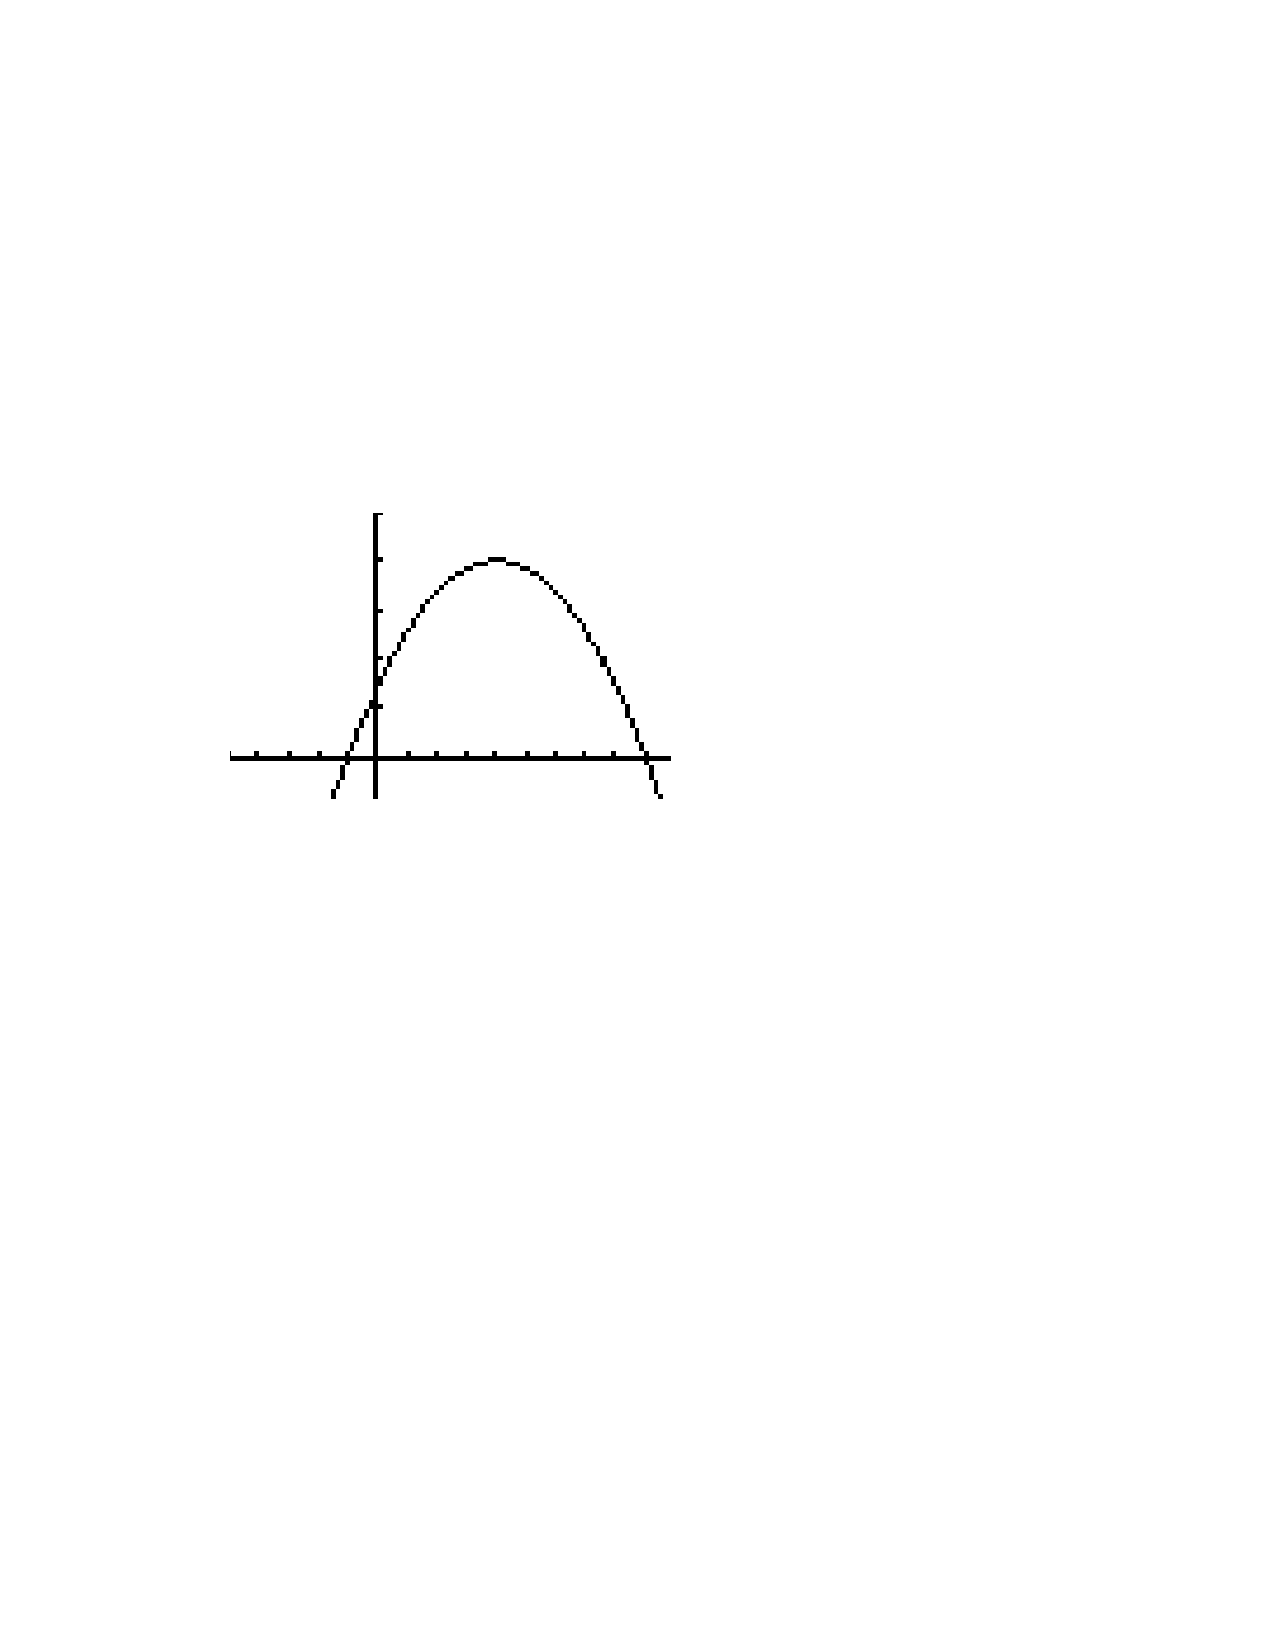
\includegraphics[trim= 170 420 250 180]{Figure1.pdf}
%\end{image}


\newcommand{\RR}{\mathbb R}
\renewcommand{\d}{\,d}
\newcommand{\dd}[2][]{\frac{d #1}{d #2}}
\renewcommand{\l}{\ell}
\newcommand{\ddx}{\frac{d}{dx}}
\newcommand{\dfn}{\textbf}
\newcommand{\eval}[1]{\bigg[ #1 \bigg]}

\usepackage{multicol}

\renewenvironment{freeResponse}{
\ifhandout\setbox0\vbox\bgroup\else
\begin{trivlist}\item[\hskip \labelsep\bfseries Solution:\hspace{2ex}]
\fi}
{\ifhandout\egroup\else
\end{trivlist}
\fi} %% we can turn off input when making a master document

\title{Recitation \#28 - 6.1 Velocity and Net Change}  

\begin{document}
\begin{abstract}		\end{abstract}
\maketitle

\section*{Warm up:} 
If the velocity of an object moving along a straight line is positive, does the displacement of the object equal the distance the object traveled?  Why or why not?
		\begin{freeResponse}
		Yes, if the velocity is positive then $\left| v(t) \right|=v(t)$.  Then (informally)
			\begin{equation*}
			\text{displacement } = \int_a^b v(t) \d t = \int_a^b \left| v(t) \right| \d t = \text{ distance traveled}.
			\end{equation*}
		\end{freeResponse}	
		
		
		

	
	
	
	
	

\section*{Group work:}



%problem 1
\begin{problem}
Solve the following word problems:

	\begin{enumerate}
	
	%part a
	\item  The velocity function for a man walking along a straight road which runs east and west is given by 
	$v(t) = -t^2 + 4t - 3$ feet per minute.
		
		\begin{enumerate}
		
		%part ai
		\item[i.]  Find the total displacement the man traveled from $2$ minutes to $6$ minutes (assume east is positive). 
			\begin{freeResponse}
			The man's total displacement is given by $\int_2^6 v(t) \d t$.  So we compute:
				\begin{align*}
				\int_2^6 v(t) \d t &= \int_2^6 (-t^2 + 4t - 3) \d t  \\
				&= \eval{- \frac{1}{3} t^3 + 2t^2 - 3t}_2^6  \\
				&= (-72 + 72 - 18) - \left( - \frac{8}{3} + 8 - 6 \right)  \\
				&= \frac{8}{3} - 20 = - \frac{52}{3}.
				\end{align*}
			So the man's displacement is $\frac{52}{3}$ feet west of his original location.
			\end{freeResponse}
				
		%part aii
		\item[ii.]  Find the total distance the man traveled from $2$ minutes to $6$ minutes. 
			\begin{freeResponse}
			First notice that $v(t) = -(t^2 - 4t + 3) = -(t-1)(t-3)$.  So we can see that
				\begin{align*}
				v(t) &> 0 \text{ when }  2 \leq t < 3.  \\
				v(t) &< 0 \text{ when } 3 < t \leq 6.
				\end{align*}
			Thus, the total distance that the man traveled from $2$ minutes to $6$ minutes is:
				\begin{align*}
				\int_2^6 \left| v(t) \right| \d t &= \int_2^3 \left| v(t) \right| \d t + \int_3^6 \left| v(t) \right| \d t  \\
				&= \int_2^3 v(t) \d t + \int_3^6 - v(t) \d t  \\
				&= \int_2^3 (-t^2 + 4t - 3) \d t - \int_3^6 (-t^2 + 4t - 3) \d t  \\
				&= \eval{- \frac{1}{3} t^3 + 2t^2 - 3t}_2^3 - \eval{- \frac{1}{3} t^3 + 2t^2 - 3t}_3^6  \\
				&= \left( (-9+18-9) - (- \frac{8}{3} + 8 - 6) \right) -  \\
				& \left( (-72+72-18)-(-9+18-9) \right)  \\
				&= \left(0 - 2 + \frac{8}{3} \right) - \left( -18 - 0 \right)  \\
				&=  16 + \frac{8}{3} = \frac{56}{3}.
				\end{align*}
			So, the total distance that the man traveled is $\frac{56}{3}$ feet.
			\end{freeResponse}
				
		%part aiii
		\item[iii.]  Suppose that the man's position $2$ minutes into the trip is $5$ feet east of his mailbox.  What is his position (relative to his mailbox) at $6$ minutes.
			\begin{freeResponse}
			$s(6) = s(0) + \int_2^6 v(t) \d t = 5 + \left(- \frac{52}{3} \right) = - \frac{37}{3}. $
			
			So the man's position at $6$ minutes is $\frac{37}{3}$ feet west of his mailbox.
			\end{freeResponse}
				
		\end{enumerate}
		
		
		
	%part b
	\item  Sammy the Snail sets up camp in the median of I-70 and, starting at noon and ending at 6pm, hikes back and forth along the highway.  He starts his hike at his campsite.  His velocity at time $t$ hours (after noon)  is given by $v(t)=(t-2)(t-5)$ inches per hour.  Find the total distance Sammy travelled on his hike.  
		\begin{freeResponse}
		The total distance that Sammy travels is $\int_0^6 \left| v(t) \right| \d t$.  
		The following picture indicates where $v(t)$ is positive and negative:
			\begin{image}
			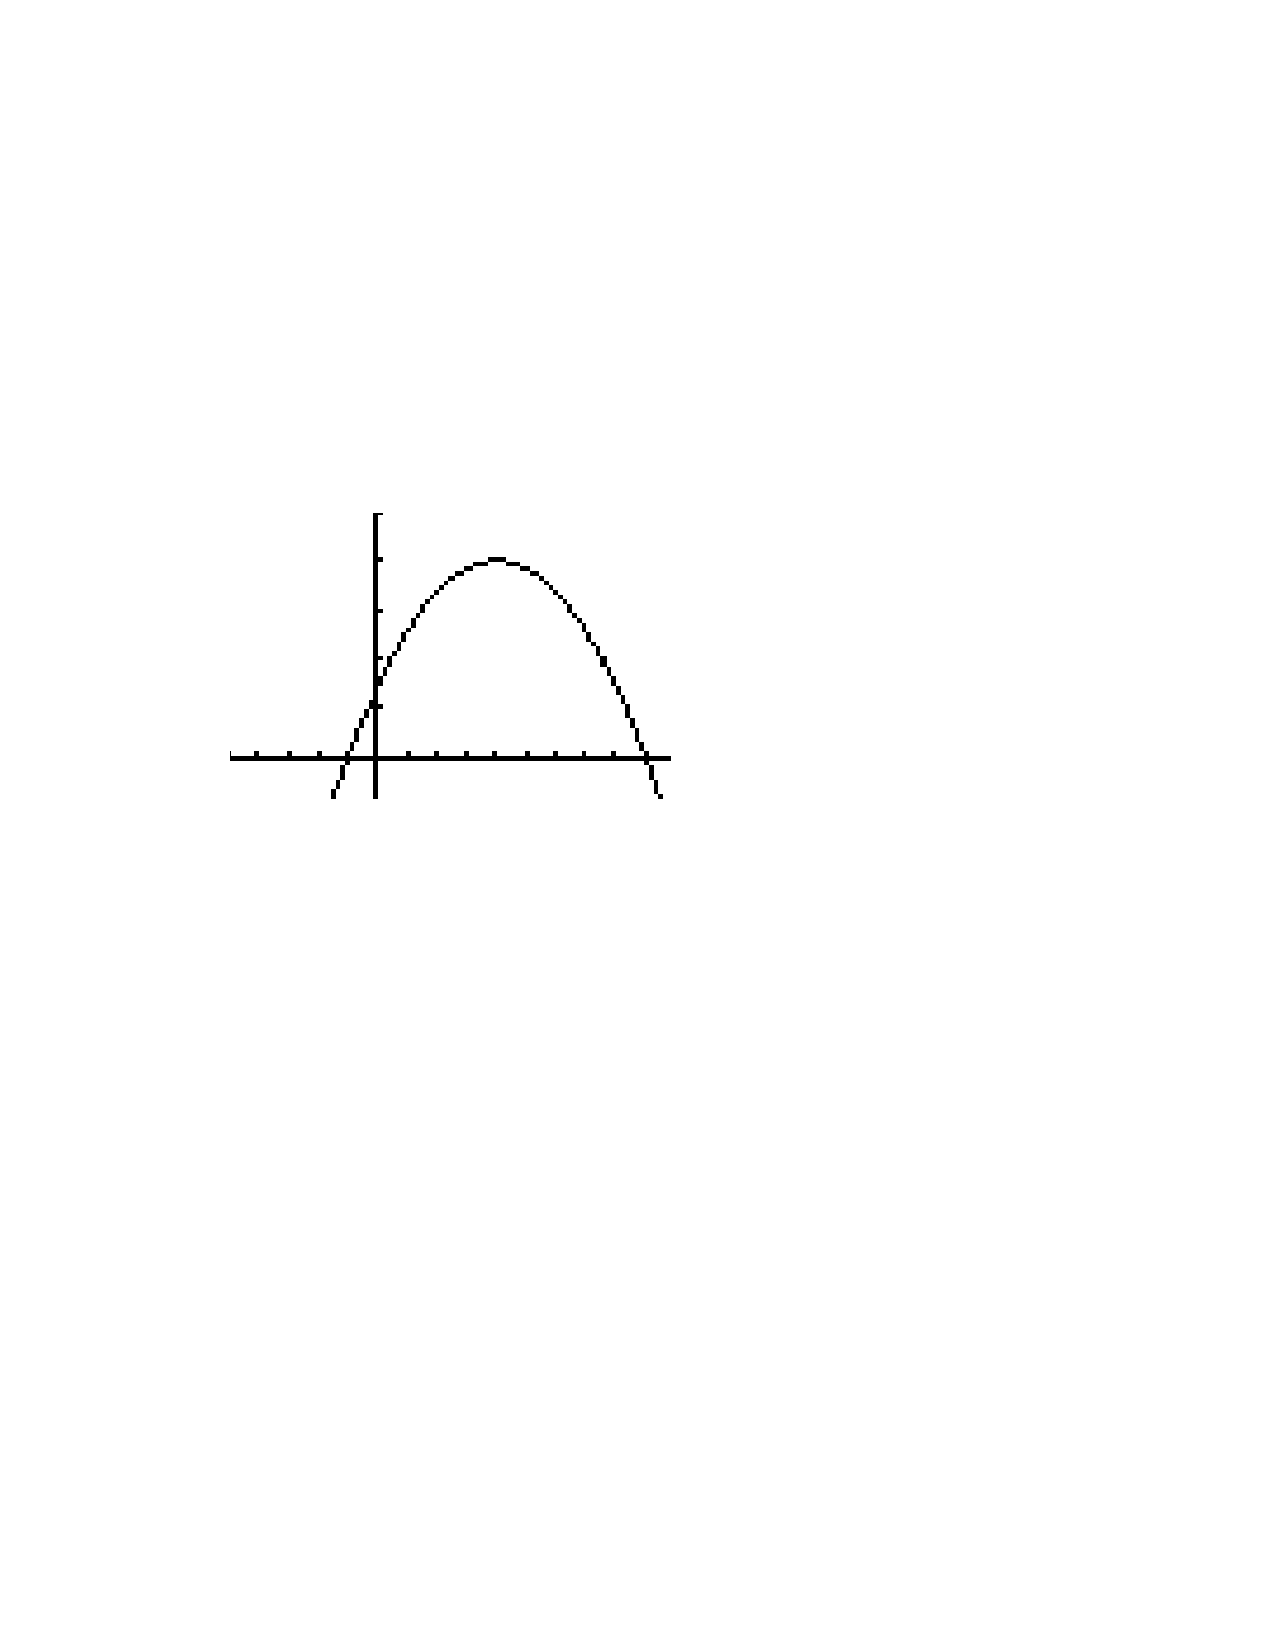
\includegraphics[trim= 170 400 250 290]{Figure1.pdf}
			\end{image}
		So we compute:
			\begin{align*}
			\int_0^6 \left| v(t) \right| \d t &= \int_0^2 \left| v(t) \right| \d t + \int_2^5 \left| v(t) \right| \d t + \int_5^6 \left| v(t) \right| \d t  \\
			&= \int_0^2 v(t) \d t - \int_2^5 v(t) \d t + \int_5^6 v(t) \d t  \\
			&= \int_0^2 (t^2 - 7t + 10) \d t - \int_2^5 (t^2 - 7t + 10) \d t + \int_5^6 (t^2 - 7t + 10) \d t  \\
			&= \eval{\frac{1}{3}t^3-\frac{7}{2}t^2+10t}_0^2-\eval{\frac{1}{3}t^3-\frac{7}{2}t^2+10t}_2^5+\eval{\frac{1}{3}t^3-\frac{7}{2}t^2+10t}_5^6  \\
			&= \left( \left(\frac{8}{3}-14+20 \right)-0\right)-\left( \left( \frac{125}{3}-\frac{175}{2}+50 \right)-\left( \frac{8}{3}+6 \right) \right)+  \\
			&\left( \left( 72-126+60 \right) - \left( \frac{125}{3} - \frac{175}{2} + 50 \right) \right)  \\
			&= -82+175-78=15.
			\end{align*}
		So Sammy has traveled a distance of $15$ inches.
		\end{freeResponse}
		
		
		
	\end{enumerate}
		
		
\end{problem}





\newpage




%problem 2
\begin{problem}
Assume that the {\it rate of change} (in dollars per day) of the price of shares of stock 
in the WeSaySo Company (with $t$ in days) is modeled by the equation $r(t) = -3t^2+30t-63$ 
(note that this is technically a {\it discrete} function, but prices change so often with stocks that modeling this with a continuous function makes sense).  
Assume also that the price of a share of stock on day $1$ (i.e., $t=1$) is $\$51$.  
Answer the following questions:
	\begin{enumerate}
	
	\item  Find the rate of change of price at $t=5$.  
		\begin{freeResponse}
		$r(5) = -3(25) + 30(5) - 63 = -75+150-63=12 \text{ dollars/day}$.  
		\end{freeResponse}
		
		
		
	
	\item  Find the price of a share of stock at $t=5$.  
		\begin{freeResponse}
		Let $p(t)$ denote the price of a share of stock at any time $t$.  
		Then notice that $r(t) = p^\prime (t)$.  
		We will first find $p(t)$ for general $t$, and then substitute $t=5$ to solve this problem.
			\begin{align*}
			p(t) &= \int_1^t r(s) \d s + p(1)  \\
			&= \int_1^t \left( -3s^2 + 30s - 63 \right) \d s + 51  \\
			&= \eval{ - s^3 + 15s^2 - 63s}_1^t + 51  \\
			&= \left( - t^3 + 15t^2 - 63t \right) - (-1+15-63) + 51  \\
			&= -t^3 + 15t^2 - 63t + 100.
			\end{align*}
		So, $p(5) = -125+375-315+100=35\$.$
		\end{freeResponse}
		
		
		
	
	\item  How fast is the rate of change of price changing at $t=5$?  
		\begin{freeResponse}
		$r'(t) = -6t + 30$.  So, $r'(5) = -30+30=0$.  
		\end{freeResponse}
		
		
		
	
	\item  How much did the price of a share of stock change in the first $6$ days (i.e., on $[1,6]$)?  
		\begin{freeResponse}
		$p(6) - p(1) = (-216+540-378+100) - 51 = -5\$. $
		\end{freeResponse}
		
		
		
	
	\item  What was the greatest rate of change of price during the first $6$ days (i.e., on $[1,6]$)?  
		\begin{freeResponse}
		This question wants us to maximize $r(t)$ on the closed interval $[1,6]$.  
		So we need to find all critical points of $r(t)$ on $[1,6]$.  
		$$ r'(t) = -6t+30:=0 \quad \Longrightarrow \quad t=5  $$
		Then, using the closed interval method, we simply plug $t=1,5,6$ into $r(t)$ and check which has the greatest output.  
			\begin{align*}
			&r(1) = -3+30-63=-36  \\
			&r(5) = -75+150-63=12  \\
			&r(6) = -108+180-63=9.
			\end{align*}
		Thus, the greatest rate of change of price is $12$ dollars/day when $t=5$.  
		\end{freeResponse}
		
		
		
	
	\item  What was the greatest price of a share of stock during the first $6$ days (i.e., on $[1,6]$)?  
		\begin{freeResponse}
		This question wants us to maximize $p(t)$ on the closed interval $[1,6]$.  
		So we need to find all critical points of $p(t)$ on $[1,6]$. 
		But note that $p'(t) = r(t)$.  So critical points of $p(t)$ are just roots of $r(t)$.  
		$$ r(t) = 0 $$
		$$ -3t^2+30t-63 = 0 $$
		$$ -3(t^2-10t+21)=0 $$
		$$ -3(t-3)(t-7) = 0 $$
		$$ t=3,7 \quad \Longrightarrow \quad t=3 $$
		since $7$ is not in the interval $[1,6]$.  
		So we again use the closed interval method:
			\begin{align*}
			&p(1) = -1+15-63+100 = 51  \\
			&p(3) = -27 + 135 - 189 + 100 = 19  \\
			&p(6) = -216+540-378+100=46  \\
			\end{align*}
		Thus, the greatest price of the stock is $\$51$ when $t=1$.  
		\end{freeResponse}

		
		
		
	
	\end{enumerate}


\end{problem}



	
	
	
	
	
	
	
	
			
			

%problem 3
\begin{problem}
Evaluate the following integrals:

	\begin{enumerate}
	
	%part a
	\item  $\int \frac{13x^7}{\sqrt{3x^4-5}} \d x$
		\begin{freeResponse}
		Let $v = 3x^4 - 5$.  Then
			\begin{align*}
			&\d v = 12 x^3 \d x  \\
			&x^4 = \frac{1}{3} (v + 5).
			\end{align*}
		So
			\begin{align*}
			\int \frac{13x^7}{\sqrt{3x^4-5}} \d x &= \frac{13}{12} \int \frac{(x^4)(12 x^3)}{\sqrt{3x^4-5}} \d x  \\
			&= \frac{13}{12} \int \frac{\frac{1}{3} (v+5)}{\sqrt{v}} \d v  \\
			&= \frac{13}{36} \int \left( v^{\frac{1}{2}} + 5v^{-\frac{1}{2}} \right) \d v  \\
			&= \frac{13}{36} \left( \frac{2}{3} v^{\frac{3}{2}} + 10 v^{\frac{1}{2}} \right) + C  \\
			&= \frac{13}{54} (3x^4-5)^{\frac{3}{2}} + \frac{65}{18} \sqrt{3x^4 - 5} + C.
			\end{align*}
		\end{freeResponse}
		
		
		
	%part b
	\item  $\int \frac{x^3}{x^2 - 3} \d x$
		\begin{freeResponse}
		Let $w = x^2 - 3$.  Then
			\begin{align*}
			&\d w = 2x \d x  \\
			&x^2 = w + 3.
			\end{align*}
		So
			\begin{align*}
			\int \frac{x^3}{x^2 - 3} \d x &= \frac{1}{2} \int \frac{(x^2)(2x)}{x^2 - 3} \d x  \\
			&= \frac{1}{2} \int \frac{w+3}{w} \d w  \\
			&= \frac{1}{2} \int \left(1 + \frac{3}{w} \right) \d w  \\
			&= \frac{1}{2} \left( w + 3 \ln|w| \right) + C  \\
			&= \frac{1}{2} \left( x^2 - 3 + 3\ln|x^2-3| \right) + C.
			\end{align*}
		\end{freeResponse}
		
		
		
	\end{enumerate}
			
			
	
\end{problem}
















%problem 2
\begin{problem}
\dfn{Practice Problem:}  Suppose that $r(t) = r_0 e^{-kt}$ (with $k>0$) is the rate at which a nation extracts oil.  
The current rate of extraction is $r(0) = 10^7$ barrels/yr.  
Also assume that the estimate of the total oil reserve (ie, the amount of oil remaining beneath the ground in this country) is $2 \times 10^9$ barrels.

	\begin{enumerate}
	
	%part a
	\item  Find $Q(t)$, the total amount of oil extracted by the nation after $t$ years.
		\begin{freeResponse}
		$Q(t) = Q(0) + \int_0^t r(s) \d s$.  Note that $Q(0)=0$ since no oil will have been extracted in $0$ time.  So
			\begin{align*}
			Q(t) &= \int_0^t r(s) \d s  \\
			&= \int_0^t r_0 e^{-ks} \d s  \\
			&= - \frac{r_0}{k} \eval{e^{-ks}}_0^t  \\
			&= - \frac{r_0}{k} \left( e^{-kt} - 1 \right)  \\
			&= - \frac{1}{k} 10^7 \left(e^{-kt}-1 \right)  \\
			\end{align*}
		\end{freeResponse}
		
		
		
	%part b
	\item  Evaluate $\lim_{t \to \infty} Q(t)$ and explain the meaning of this limit.
		\begin{freeResponse}
			\begin{align*}
			\lim_{t \to \infty} Q(t) &= \lim_{t \to \infty} - \frac{1}{k} 10^7 \left(e^{-kt}-1 \right)  \\
			&= - \frac{1}{k} 10^7 (0-1)  \\
			&= \frac{1}{k} 10^7.
			\end{align*}
		\end{freeResponse}
		
		
		
	%part c
	\item  Find the minimum decay constant $k$ for which the total oil reserves will last forever.
		\begin{freeResponse}
		For the oil reserves to last forever, we need that
			\begin{align*}
			&\lim_{t \to \infty} Q(t) \leq 2 \times 10^9  \\
			 &\Longleftrightarrow \qquad \frac{1}{k} 10^7 \leq 2 \times 10^9  \\
			 &\Longleftrightarrow \qquad \frac{1}{k} \leq 2 \times 10^2 = 200  \\
			 &\Longleftrightarrow \qquad \frac{1}{200} \leq k.
			\end{align*}
		So the minimum value for $k$ is $\frac{1}{200}$.  
		\end{freeResponse}
		
		
		
	%part d
	\item  Suppose that the decay constant is half the minimum value found in part (c).  
	How long will the total oil reserves last?
		\begin{freeResponse}
		First note that $k = \frac{1}{2} \cdot \frac{1}{200} = \frac{1}{400}$.  
		We want to find the value of $t$ such that:
			\begin{equation*}
			Q(t) = 2 \times 10^9
			\end{equation*}
			\begin{equation*}
			- 400 \times 10^7 \left(e^{-\frac{1}{400}t}-1 \right) = 2 \times 10^9
			\end{equation*}
			\begin{equation*}
			\left(e^{-\frac{1}{400}t}-1 \right) = \frac{2 \times 10^9}{-400 \times 10^7} = - \frac{1}{2}
			\end{equation*}
			\begin{equation*}
			e^{-\frac{1}{400}t} = \frac{1}{2}
			\end{equation*}
			\begin{equation*}
			-\frac{1}{400}t=\ln \left(\frac{1}{2} \right) = -\ln(2)
			\end{equation*}
			\begin{equation*}
			t = 400 \ln(2) \approx 277.259 \text{ years}.
			\end{equation*}
		\end{freeResponse}
		
		
		
	\end{enumerate}
		
		
		

\end{problem}




















	
	
	
	
	
	
	
	
	

	










								
				
				
	














\end{document} 


















